%\chapter{Etude des besoins et contraintes dans les visites touristiques}
\chapter{Les enjeux de l'interaction dans les visites touristiques}
\label{chap:etude}

L'objectif de ce travail de thèse est de répondre aux problématiques d'accès à l'information durant les visites touristiques. 
Ce chapitre va étudier en détail les besoins et les attentes des musées et des visiteurs dans le cadre des nouveaux types d'interaction existants à l'heure actuelle.
En s'intéressant notamment à une interaction à base de gestes, développée grâce à une étude utilisateur réalisée avec des séances participatives.

Les raisons de créer de nouveaux moyens d'interaction dans les musées sont multiples (section~\ref{sec:nouveauxmoyendinteraction}), ce qui implique de réfléchir à de nouvelles méthodes d'accès à l'information. 
Le projet GUIMUTEIC (section~\ref{sec:GUIMUTEIC}) doit répondre à ces besoins, tout en respectant ses contraintes de déploiement. 


\section{Les nouveaux moyens d'interaction et d'accès à l'information muséale}
\label{sec:nouveauxmoyendinteraction}

Les professionels des musées, ainsi que les visiteurs, ont vu leur compréhension de ce qu'est un musée changer, avec l'introduction de nouvelles technologies au sein des musées~\cite{knell2010shape}.
Le problème des nouvelles interactions n'est pas que technologique, il nécessite une étude interdisciplinaire des intéractions sociales et technologiques dans les musées, comme le souligne le ``museum informatics'' défini par Marty~\cite{marty2008museum}.


L'essor des sciences de l'information et des technologies a créé de nouveaux moyens d'accès et de traitement de l'information dans les musées, et une nouvelle manière de penser les musées est apparue~\cite{marty2011my}. 
Les musées ont traditionnellement servi de recueil d'objets, dans le but de les préserver, de les étudier ou d'éduquer. 
Cependant, ils ne sont pas là uniquement pour stocker des objets.
Même si la partie fondamentale d'un musée reste sa collection d'œuvres et d'objets, la grande quantité d'information disponible à propos de chacun de ces objets est tout aussi importante~\cite{greenhill1992museums}.
Les visiteurs s'attendent aujourd'hui à avoir un accès instantané à toutes les connaissances du musée à propos de chaque œuvre. Pour rendre cela possible, il a été établi depuis longtemps que les musées se devaient de proposer de nouveaux moyens de gérer l'information~\cite{keene1996becoming}.
Chaque visiteur est unique, avec des attentes différentes, et ce qu’il retiendra d'une visite va dépendre des objets vus, du personnel du musée, du contexte socioculturel et de certains aspects propres à la personne~\cite{falk2016identity}.
Il est important d'avoir une personnalisation de la visite pour que chacun puisse avoir la meilleure expérience, adaptée à ces besoin.
Par exemple, le projet PIL~\cite{kuflik2011visitor} propose une réflexion sur comment adapter le musée au visiteur, grâce aux outils technologiques, tout en faisant en sorte que celui-ci soit concentré sur les expositions et non pas sur les appareils de visites.
Il faut notamment faire attention à ce que les outils technologiques ne bloquent pas la communication avec les autres visiteurs. Ils ne doivent pas être invasifs pendant la visite, pour que l'utilisateur puisse se concentrer sur les œuvres.
 
Il est commun aujourd'hui d'avoir un audio-guide (ou un visio-guide) dans les musées afin d'avoir une audio(visio)-description d'une œuvre d'art, son impact sur la visite n'est donc pas à négliger.
Les guides permettent de garder les utilisateurs plus longtemps à l'intérieur du musée, en passant plus de temps à étudier les oeuvres, tout en s'intéressant à davantage d'oeuvres~\cite{lanir2013influence}. 
Ils permettent également d'améliorer l'interaction avec l'utilisateur~\cite{evans1999portable} ainsi que de renforcer le côté éducatif de la visite~\cite{woodruff2002eavesdropping}.
Cependant, les guides électroniques ont tendance à fermer les personnes à l'interaction sociale~\cite{angliss2006talking}. Dans le cas de visites en groupes, les appareils mobiles forcent l'utilisateur à regarder l'écran et à ne pas faire attention aux personnes avec lesquelles il est venu~\cite{grinter2002revisiting, petrelli2005user}.
Il devient également fréquent d'avoir accès à l'information directement sur son smartphone.
Ceux-ci ont le problème de couper le visiteur de ce qui l'entoure, car il va regarder son téléphone plutôt que ce qui l'entoure. Comme il est devenu clair qu'il était difficile de détourner une personne de son smartphone, celui-ci peut être utilisé par le musée pour guider le visiteur ou fournir un plus à la visite~\cite{gammon2008designing, pierroux2011bridging, weilenmann2013instagram}.
Pour ne pas détourner l'attention des utilisateurs envers les œuvres, ni couper le visiteur de son groupe, le projet GUIMUTEIC n'utilise pas d'écran, mais uniquement un casque audio ouvert.

Plusieurs approches modernes proposent de nouvelles interfaces technologiques, pour l'interaction avec les œuvres culturelles.
Par exemple, le ``SmartMuseum''~\cite{kuusik2009smartmuseum} propose à l'aide de capteurs RFID (Radio Frequency Identification) de donner des informations au visiteur. 
Ce dernier peut construire sa propre visite sur le site web en amont de sa venue, et reconnaître sur site les œuvres sélectionnées.
L'utilisation d'étiquettes RFID limite, ou complexifie, la modification de l'organisation du musée. Le maintien et l'organisation de la base d'étiquette devient une contrainte et demande un certain engagement de la part du musée. 
Ce système requiert l'utilisation d'un appareil mobile et de plus requiert un certain degré d'apprentissage dans son utilisation.

Une solution pour aider le visiteur est d'utiliser un appareil mobile qui sert de guide audio-visuel, comme le propose le ``Museum Wearable''~\cite{sparacino2002museum}. L'appareil utilise la connaissance de l'environnement de l'utilisateur pour lui fournir l'information sur ce qui l'intéresse à un instant donné. Ce prototype utilise uniquement la position géographique de l'utilisateur pour déterminer son environnement, or la position seule n'est pas nécessairement suffisante pour déterminer le contexte autour de l'utilisateur~\cite{schmidt1999there}.
Une caméra par exemple permet d'obtenir plus d'information, et si celle-ci est positionnée de manière à voir ce que l'utilisateur perçoit, avec une vue à la première personne. On est alors capable d'avoir une information précise sur l'environnement direct.

Pour déterminer ce qui intéresse le visiteur, des méthodes d'interaction à base de gestes ont été développées. 
L'approche à base de systèmes portatifs avec vision à la première personne~\cite{baraldi2015gesture} permet de voir ce que l'utilisateur perçoit, de réagir à ces gestes et d'avoir des informations précises sur son environnement. 
Comme montré sur la figure~\ref{fig:exempleGestea}, un utilisateur, équipé de lunettes avec caméra embarquée, peut interagir avec celles-ci grâce à une série de gestes prédéfinis (figure~\ref{fig:exempleGesteb}). 
Ici les gestes sélectionnés sont Approuver (``OK''), Désapprouver (``Dislike''), Défiler (``Slide''), Valider (``Like''), Pointer et Prendre une photo (``Take a picture'').
Ces gestes n'ont cependant pas été développés avec une étude utilisateur.
Ce type d'approches permet de dépasser les limitations des appareil mobiles qui requièrent une manipulation et qui détourne l'attention de l'utilisateur des œuvres. 
Ceci permet également de proposer de nouvelles expériences d'interaction, et d'encourager le visiteur à interagir avec les œuvres, comme ils le feraient devant un guide humain. 
Si de tels gestes sont utilisés, il faut cependant étudier l'utilité des gestes reconnus, et lesquels sont les plus à même de correspondre aux attentes des utilisateurs. 
Il faut ensuite déterminer à quelle moment de la visite réaliser la reconnaissance d'environnement de l'utilisateur, et notamment reconnaître les œuvres en face de lui, pour lui fournir une réponse à son interaction.


\begin{figure}[htbp]
\begin{subfigure}{0.49\textwidth}
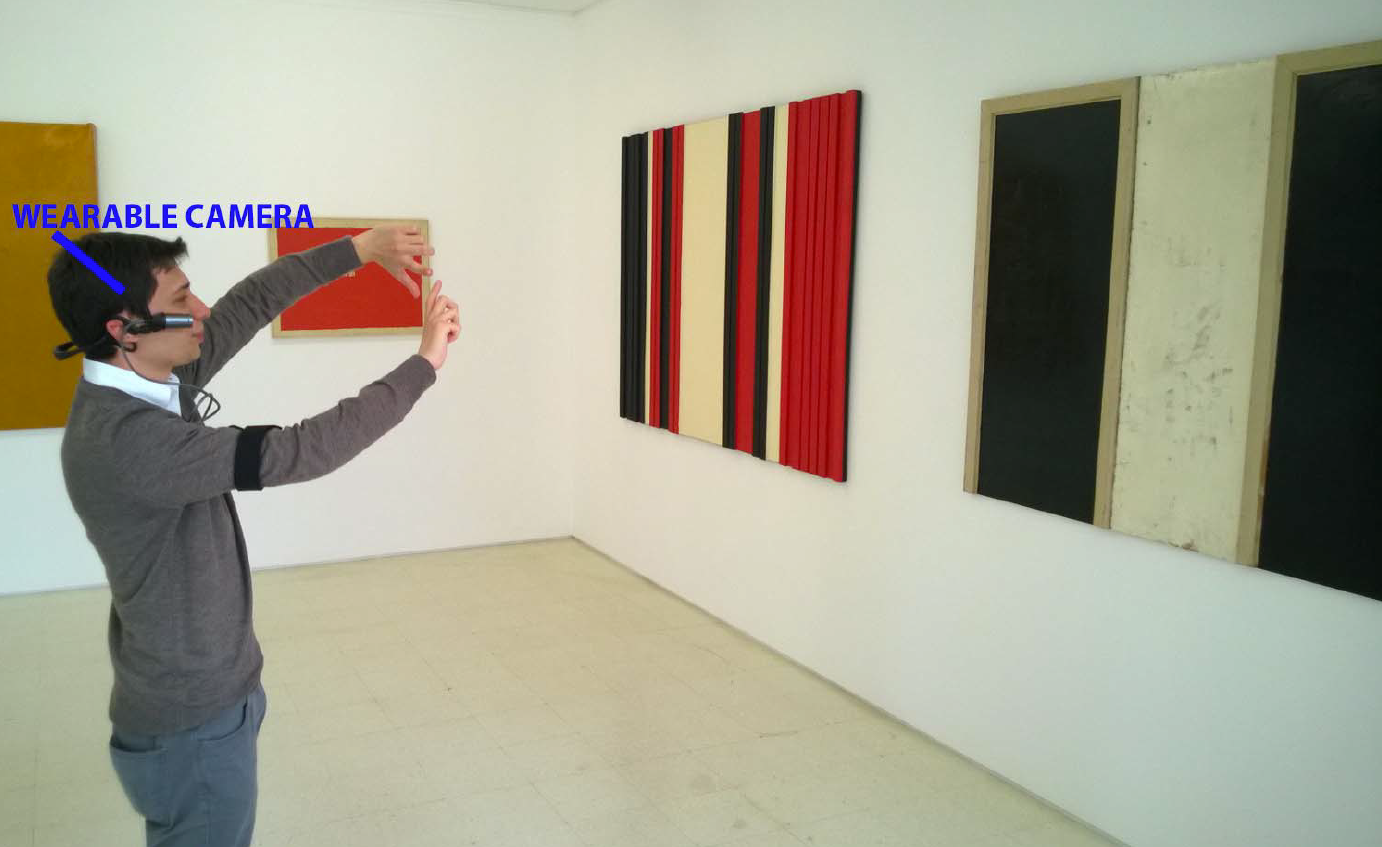
\includegraphics[width=\linewidth]{figures/wearable.PNG}
\caption{Geste en face d'une oeuvre} \label{fig:exempleGestea}
\end{subfigure}
\hspace*{\fill} % separation between the subfigures
\begin{subfigure}{0.49\textwidth}
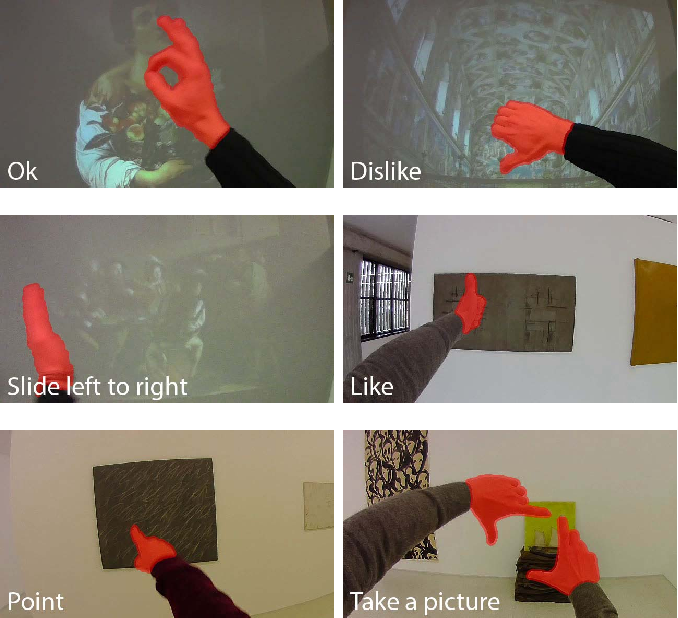
\includegraphics[width=\linewidth]{figures/gesteBaradli.png}
\caption{Gestes selectionnés} \label{fig:exempleGesteb}
\end{subfigure}
\caption{Exemple d'un système basé sur l'interaction à base de geste dans un musée~\cite{baraldi2015gesture}} \label{fig:exempleGeste}
\end{figure}




%%%%%%%%%%%%%%%%%%%%%%%%%%%%%%%%%%%%%%%%%%%%%%%%%%%%%%%%%%%
%
%   Le système GUIMUTEIC
%
%%%%%%%%%%%%%%%%%%%%%%%%%%%%%%%%%%%%%%%%%%%%%%%%%%%%%%%%%%%
\section{Le système GUIMUTEIC}
\label{sec:GUIMUTEIC}

Le système GUIMUTEIC est un système mobile, doté d'une caméra, aidant et améliorant la visite de musées. 
Pour cela, il doit être capable d'identifier les actions de l'utilisateur, et de réagir à ses besoins. 
Il doit également pouvoir reconnaître l'environnement de ce dernier, pour le guider et lui apporter les informations correspondantes à ce qu'il regarde. 

Avec une série d'études participatives, nous avons identifié les types d'interaction adaptées au projet (paragraphe~\ref{sec:gestesGUIMUTEIC}). Ainsi, tout en respectant les contraintes liées au projet (paragraphe~\ref{sec:contraintesGUIMUTEIC}), nous avons pu mettre au point un système d'aide au visiteur qui répond à ses besoins (paragraphe~\ref{sec:systemeGUIMUTEIC}). 



%%%%%%%%%%%%%%%%%%%%%%%%%%%%%%%%%%%%%%%%%%%%%%%%%%%%%%%%%%%
%
%   Les Gestes GUIMUTEIC
%
%%%%%%%%%%%%%%%%%%%%%%%%%%%%%%%%%%%%%%%%%%%%%%%%%%%%%%%%%%%
\subsection{Une interaction à base de gestes}
\label{sec:gestesGUIMUTEIC}

Des séances participatives de conception d'un appareil d'aide à la visite de musée ont été organisées. 
Regroupant des participants de différents âges et antécédents, elles ont permis, grâce à des exercices ludiques, de définir les usages futurs du dispositif, et de mettre en avant ce que les utilisateurs finaux attendent du produit. 
Ces séances ont fait ressortir plusieurs méthodes d'interaction susceptibles d'être intéressantes pour les visiteurs.
Les détails de cette étude sont reportés dans l'annexe~\ref{sec:etudeGestes}~``\nameref{sec:etudeGestes}’’.

\`A l'issue de ces séances, l'interaction privilégiée est celle à base de gestes. Cinq gestes ont été identifiés comme utiles à l'interaction, et sont présentés dans la figure~\ref{fig:photoGestes}. Il s'agit de \textbf{pointer}, signaler \textbf{``OK''}, \textbf{valider (ou ``liker'')}, \textbf{arrêter} et \textbf{stop} (ou pause).  

\begin{figure}[!htb]
	\begin{minipage}[c]{.32\linewidth}
		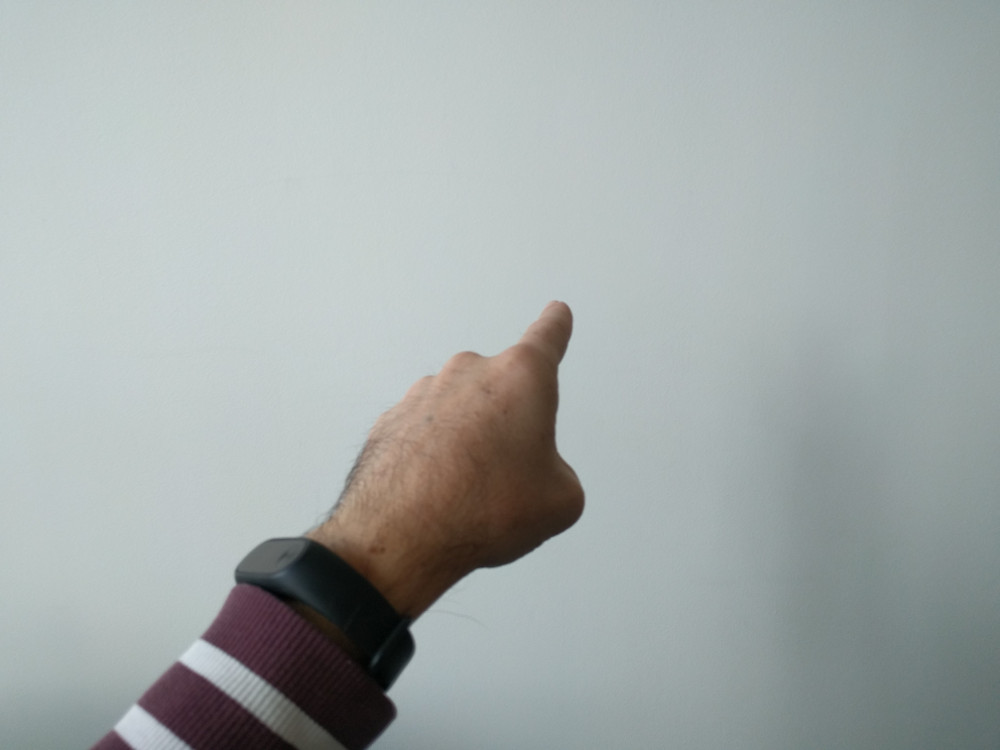
\includegraphics[width=\columnwidth]{figures/1.jpg}%
		\caption*{Pointer}%
	\end{minipage} \hfill
	\begin{minipage}[c]{.32\linewidth}
		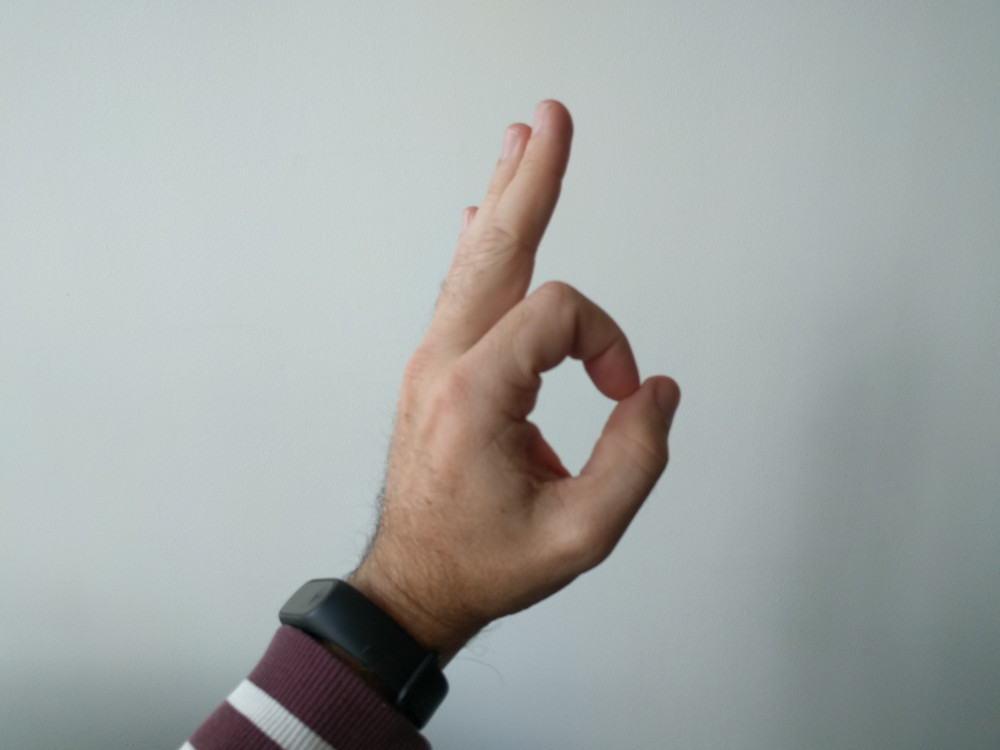
\includegraphics[width=\columnwidth]{figures/2.jpg}%
		\caption*{OK}%
	\end{minipage} \hfill
	\begin{minipage}[c]{.32\linewidth}
		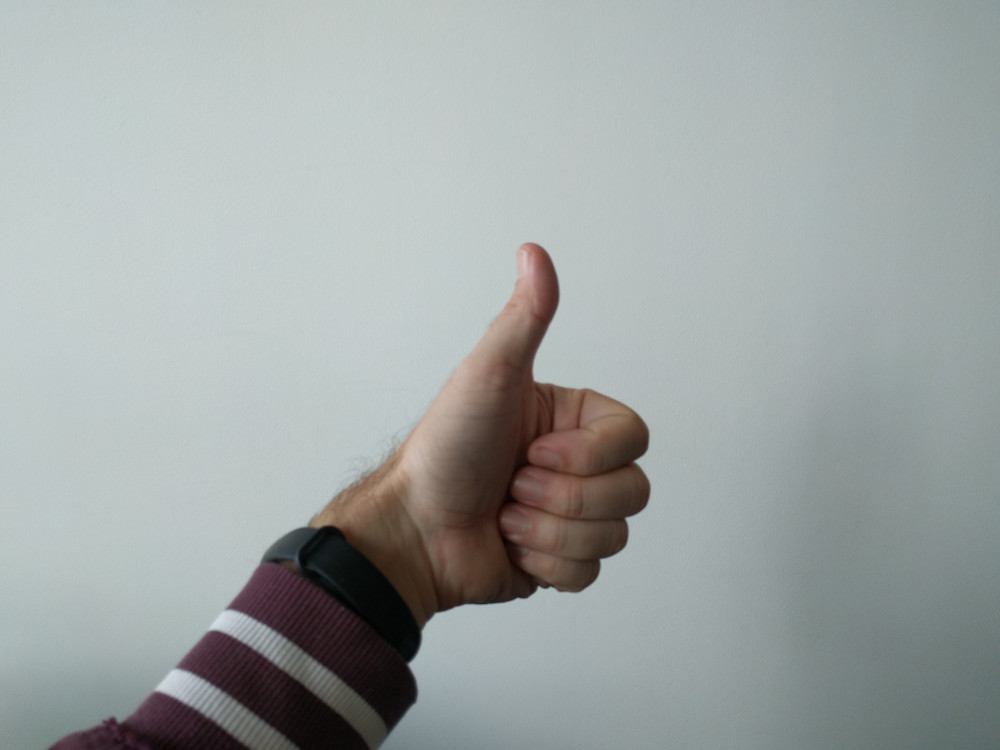
\includegraphics[width=\columnwidth]{figures/3.jpg}%
		\caption*{Valider}%
	\end{minipage}
	\centering
	\begin{minipage}[c]{.32\linewidth}
		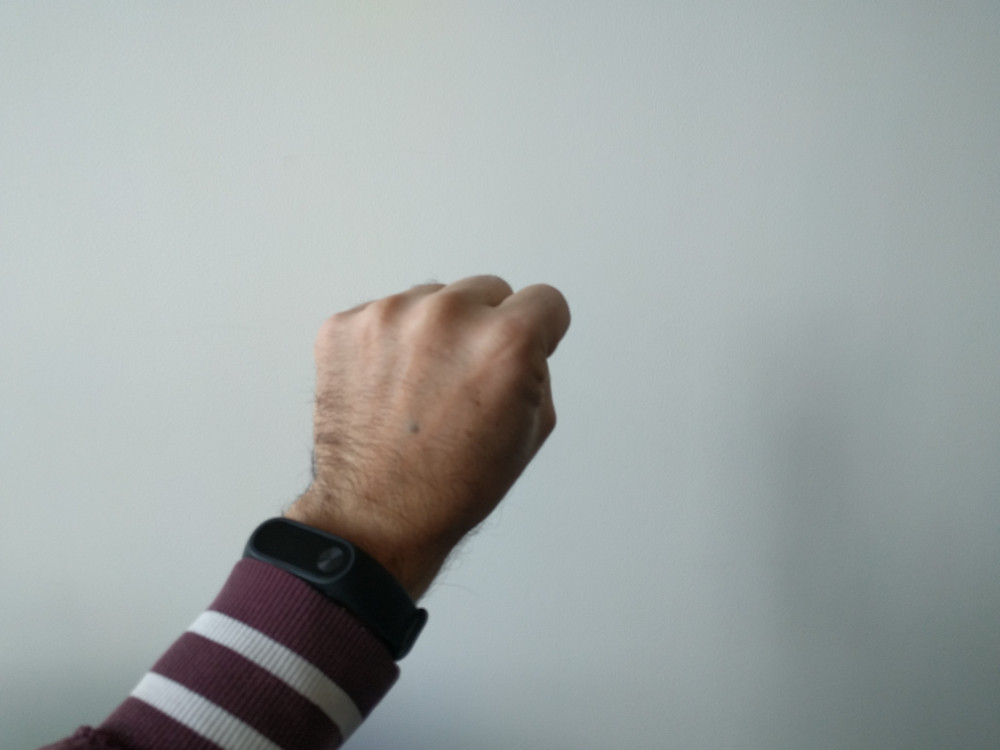
\includegraphics[width=\columnwidth]{figures/4.jpg}%
		\caption*{Arrêter}%
	\end{minipage}
	\begin{minipage}[c]{.32\linewidth}
		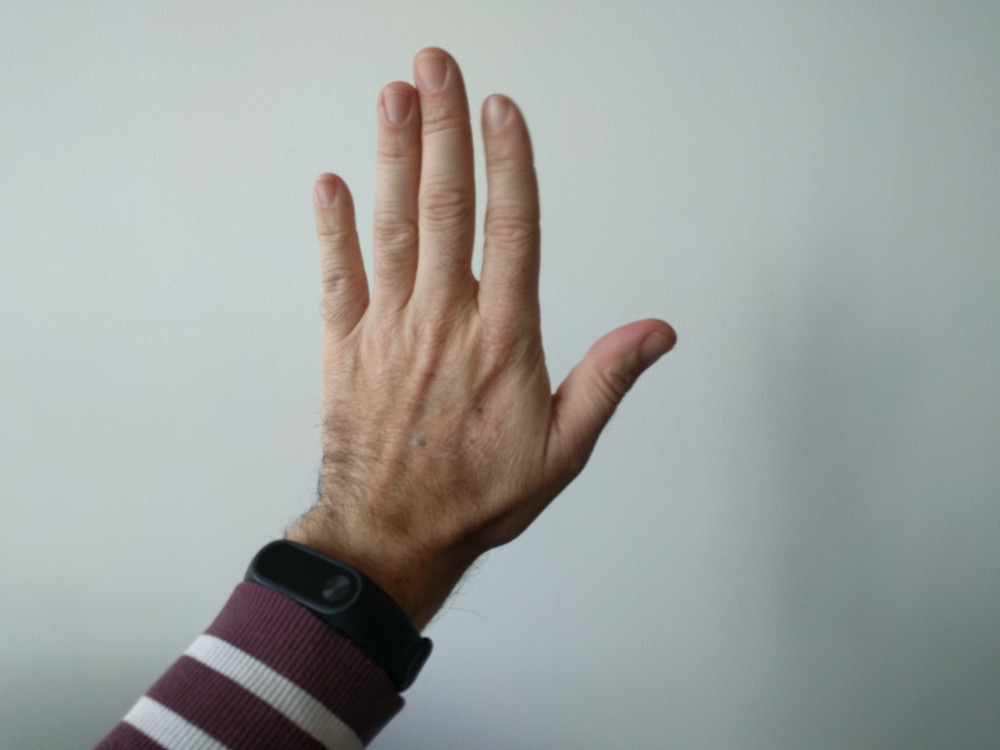
\includegraphics[width=\columnwidth]{figures/5.jpg}%
		\caption*{Stop}%
	\end{minipage}
	\caption{Les 5 gestes mis en avant par les séances de conceptions participative.}
	\label{fig:photoGestes}
\end{figure}

Pour créer un système de reconnaissance de ces gestes, un ensemble de vidéos de gestes correspondant aux attentes du projet ont été réalisés. 
Ce corpus est composé de vidéos en vue à la première personne, prise dans différentes conditions, avec des environnements différents et notamment sur fond vert. 
La description complète du corpus est fournie en annexe~\ref{sec:etudeGestes}. 
Les méthodes proposées dans le chapitre~\ref{chap:gestes} seront testées sur ce corpus.





%%%%%%%%%%%%%%%%%%%%%%%%%%%%%%%%%%%%%%%%%%%%%%%%%%%%%%%%%%%
%
%   Les Contraintes GUIMUTEIC
%
%%%%%%%%%%%%%%%%%%%%%%%%%%%%%%%%%%%%%%%%%%%%%%%%%%%%%%%%%%%
\subsection{Les contraintes des musées et du projet GUIMUTEIC}
\label{sec:contraintesGUIMUTEIC}

Le projet GUIMUTEIC est le fruit d'une collaboration industrielle, et doit donc répondre à un certain nombre de contraintes qui en découlent.
Le premier type de contraintes est lié à la distributivité du produit. Le système doit être capable d'être applicable à n'importe quel type de musée. 
Dans le cadre du projet, deux types de musées sont étudiés: un musée d'archéologie, le musée Gallo-Romain de Lyon Fourvière, et le musée d'art de Grenoble. 
Les types d'objets présents dans ces musées étant variés, leur étude nous permet de produire un système généralisable. 

Un autre facteur important de la faisabilité de ce type de projet, est le coût, en infrastructure et en heures, de l'installation du système dans un musée. 
Compte tenu de l'aspect portatif de dispositif GUIMUTEIC, il est important qu'aucune connexion permanente à un serveur ne soit nécessaire. 
En effet, la connection à un serveur distant sous-entend, en plus de la présence et de la maintenance de serveurs, une connectivité dans l'ensemble du musée. 

Pour être utilisable par le plus de personnes possible, un guide doit pouvoir être utilisé sans apprentissage de la part de la personne qui l'utilise, pour ne pas décourager celle-ci, et permettre à n'importe qui de l'utiliser de manière simple, sans formation. 
De plus, le système doit fonctionner sans apprentissage de la part du système pour chaque utilisateur. 
Il doit être capable de s'adapter à toutes les morphologies, de taille notamment, et de couleur de peau.

De la même manière, pour la mise en place de la reconnaissance d'environnements et d'œuvre autour de l'utilisateur, une base de données des lieux, œuvres et autres points d'intérêt du musée, doit d'être constituée. 
Ceci pouvant être un frein considérable à l'installation d'un nouveau système, du fait du coût en heures de prise de vues et en maintenance, nous avons de forte contraintes sur la création de cette base. 
Nous nous limitons à quelques photos par œuvre et point d'intérêt du musée. 
La capture de vidéos de visite est un processus très coûteux: en plus de l'enregistrement, qui doit faire intervenir un certain nombre de personnes pour avoir une diversité suffisante, il faut prendre en compte le coût de l'annotation de chacune de ces vidéos.
Identifier quel objet est visible à chaque instant, si possible même annoter la position de l'objet dans l'image, est long et nécessite un certain investissement, qui ne correspond pas au projet dans lequel nous nous situons.
Les propositions dans la suite de cette thèse doivent donc répondre à ces contraintes :

\begin{itemize}
	\item Quelques images par œuvre : la reconnaissance d'instance dans les images doit pouvoir se faire avec seulement quelques exemples de ladite instance comme référence.
	\item Portabilité de l'appareil : la quantité de calcul et l’utilisation de la mémoire pour le reconnaissance d'actions et d'instances doivent être aussi limités que possible, en ayant comme objectif de tout réaliser sur un processeur mobile.
	\item Pas de vidéos de visite : la réalisation de vidéos de visite complètes, annotées, demande trop d'investissement. Nous partons donc du principe que nous ne disposons pas de ce type de vidéos.
\end{itemize}





\subsection{Le système d'interaction GUIMUTEIC}
\label{sec:systemeGUIMUTEIC}

Notre approche pour la création d'une aide à la visite muséale est présentée dans le schéma~\ref{fig:actioncontexte}.
L'utilisateur, libéré de tout appareil dans ses mains, peut interagir avec le système GUIMUTEIC à travers des gestes prédéfinis.
On voit sur la figure le visiteur sur la gauche interagir avec le système GUIMUTEIC au moyen de la caméra.
A l’aide de la reconnaissance de gestes et de reconnaissance d’instance, le système peut fournir un retour d’information adapté.
Nous développons donc une approche de reconnaissance de gestes avec une caméra en vue à la première personne (chapitre~\ref{chap:gestes}, ~\nameref{chap:gestes}).
Dans le but de donner des informations au visiteur, le système doit être capable de détecter son environnement. 
Nous nous basons pour cela sur la reconnaissance de point d'intérêts dans le musée (chapitre~\ref{chap:similarite}~\nameref{chap:similarite}). 
Ces points d'intérêts sont généralement des œuvres.
Le retour d'information à l'utilisateur se fait grâce à un casque audio.
Dans le chapitre suivant, nous présentons l'état de l'art de la reconnaissance d'instances dans les images, ainsi que celui de la reconnaissance de gestes et d'actions dans les vidéos.



\begin{figure}[!htb]
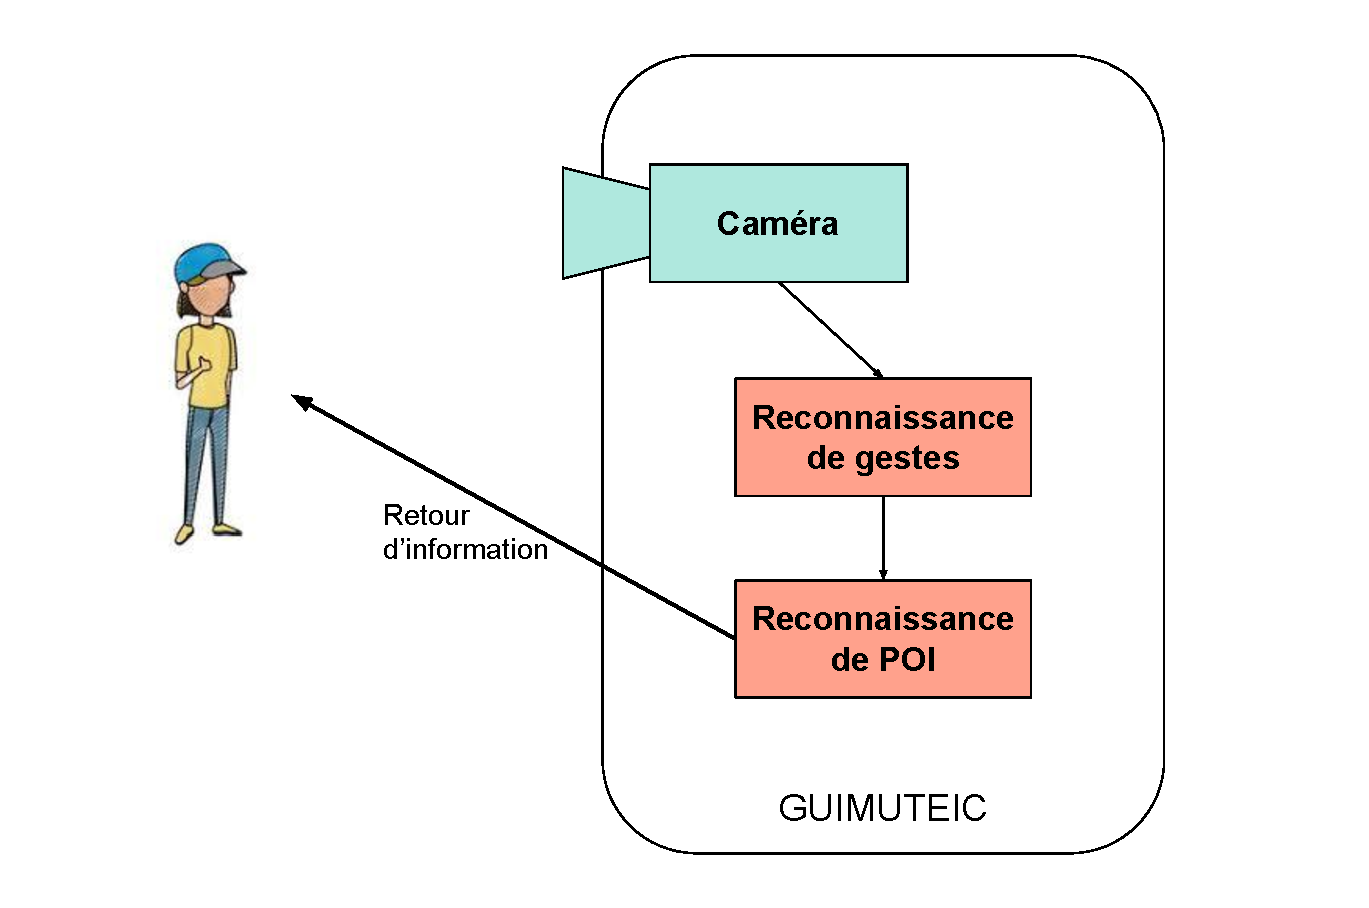
\includegraphics[width=\columnwidth]{figures/Boucledinteraction.pdf}%
\caption{Schéma d'organisation du système d'information GUIMUTEIC.}%
\label{fig:actioncontexte}%
\end{figure}


